\documentclass[10pt,letterpaper]{article}
% ========================== DO NOT MODIFY =================================== %
\usepackage[letterpaper,left=2.0cm,top=2.0cm,right=2.0cm,bottom=2.0cm]{geometry} 
\usepackage{amssymb,amsmath} % If amsmath is required
\usepackage[implicit=false]{hyperref}
\usepackage[utf8]{inputenc}
\usepackage[T1]{fontenc}
%\usepackage[USenglish]{babel} -- gives errors on many systems
\usepackage{times}
\usepackage{graphicx}
\usepackage{titling}
\usepackage{authblk}
\usepackage{multicol}
\usepackage{float}
\usepackage{enumitem}
\usepackage{booktabs}
\usepackage[small,compact]{titlesec}
\usepackage{xcolor}
\usepackage[printwatermark]{xwatermark}
% Fix titlesec for the 2.10.1 version in ubuntu 16.04
%  https://bugs.launchpad.net/ubuntu/+source/texlive-extra/+bug/1574052
\makeatletter
\@ifpackagelater{titlesec}{2016/03/21}{%
 % Package titlesec is on version 2.10.2 or higher, nothing to do %
}{%
 % Check if package titlesec is on version 2.10.1 %
 \@ifpackagelater{titlesec}{2016/03/15}{%
  % Package titlesec on version 2.10.1, patch accordingly %
  \usepackage{etoolbox}%
  \makeatletter
  \patchcmd{\ttlh@hang}{\parindent\z@}{\parindent\z@\leavevmode}{}{}%
  \patchcmd{\ttlh@hang}{\noindent}{}{}{}%
  \makeatother
 }{%
  % Package titlsecon is on version 2.10.0 or lower, nothing to do %
 }%
}
\makeatother
\titlespacing*{\section}{0pt}{5pt}{5pt}  % If you need different spacing

\usepackage[numbers,sort&compress]{natbib}
\usepackage[small,bf,tableposition=top,figureposition=bottom,skip=2pt]{caption}


% limit space between floats and text
\setlength{\textfloatsep}{10pt plus 1.0pt minus 2.0pt}
% shrink the list environments
\setlist{noitemsep}
\setlist{nolistsep}

% Shrink the bibliography
  \let\oldthebibliography=\thebibliography
  \let\endoldthebibliography=\endthebibliography
  \renewenvironment{thebibliography}[1]{%
    \begin{oldthebibliography}{#1}%
      \setlength{\parskip}{0ex}%
      \setlength{\itemsep}{0ex}%
  }%
  {%
    \end{oldthebibliography}%
  }

% Format of the front matter
\renewcommand{\Affilfont}{\small}
\setlength{\affilsep}{1ex}
\renewcommand\Authands{, }
\setlength{\droptitle}{-1.634cm}
\makeatletter
\renewcommand\AB@affilsepx{\quad\protect\Affilfont} % put affiliations into one line
\makeatother
% ============================================================================ %




%------------------------------- FRONT MATTER -------------------------------- %
\title{EIDORS Version 3.9%
\vspace{-2ex}} %remove vertical space
\author[1]{Andy~Adler}
\author[1]{Alistair~Boyle}
\author[2]{Fabian~Braun}
\author[3]{Michael~G.~Crabb}
\author[4,5]{Bart{\l}omiej~Grychtol}
\author[3]{William~R.~B.~Lionheart}
\author[3]{Henry~F.~J.~Tregidgo}
\author[6]{Rebecca~Yerworth}
\affil[1]{Carleton University, Ottawa, Canada}
\affil[2]{Centre Suisse d'Électronique et de Microtechnique, Neuchâtel, Switzerland}
\affil[3]{University of Manchester, Manchester, UK}
\affil[4]{Fraunhofer Project Group for Automation in Medicine and Biotechnology PAMB, Mannheim, Germany}
\affil[5]{University of Heidelberg, Mannheim, Germany}
\affil[6]{University College London, UK}
\date{}
%----------------------------------------------------------------------------- %



\begin{document}
\maketitle
\vspace{-1.5cm}
\thispagestyle{empty}

\begin{multicols}{2}
%\newwatermark[allpages,color=red!50,angle=45,scale=3,xpos=0,ypos=0]{DRAFT}

\noindent {\bf Abstract:}
This paper announces the release of version 3.9 of the
EIDORS software suite. We review its new features, and 
discusses its growth and citations.

\section{Introduction}
We proudly announce the release of EIDORS version 3.9,
for the 18th Int.\ Conf.\ on Biomedical Applications of EIT,
in June 2017.
The software is available at \href{www.eidors.org}{eidors.org}\, and licensed under the GNU GPLv2 or GPLv3. Archived versions are now available on Zenodo
\cite{eidors3p9} (and v3.8 \cite{eidors3p8}).


EIDORS aims to provide free software algorithms for forward modelling
and inverse solutions
of Electrical Impedance and (to some extent) Diffusion-based Optical Tomography, in
medical, industrial and geophysical settings and to share data and promote
collaboration.

\section{New Features}
Release 3.9 of EIDORS builds upon a strong foundation in reconstruction
algorithms, adding and improving a number of aspects.
\begin{itemize}
\item Faster forward solve times for real conductivity distributions

\item Improved support for GREIT reconstructions in 3D \cite{grychtol2016}

\item Improved testing framework esp.\ for core solver algs

\item New hyperparameter selection approaches \cite{braun2017}

\item Interface to ``Regularization Toolbox'' \cite{hansen2007}

\item Gmsh-based human 3D model interface \cite{grychtol2016}

\item Correction of artefacts caused by low frame rates \cite{yerworth2016}

\item Improved support for mixed point and CEM electrode models

%  - 5358 model reduction: added tutorial for diodes: model reduction from fem to resistor mesh

\item Support for 2$\frac{1}{2}$D solvers (including a rank-1 2$\frac{1}{2}$D movement Jacobian)
   \cite{boyle2016model2p5}

\item Forward solve supporting model reduction (i.e.\ efficient
       precalculation of out-of-field regions) \cite{adler2016model}

%  - improved swisstom and draeger file loaders
%  - 5288 new 2.5D rank-1 movement jacobian


\item Improved support for geophysical FEM models
%  - mk geophysics model improvements
%  - efficiency improvements
%  - 5266 Serial correct files added to R_yerworth folder
%  - 5218 l-curve/GCV hyperparameter


\item Improved support for Octave

\item Updated ability to load recent device file formats including
       auxiliary data (Dr\"ager and Swisstom formats)




\item Expanded shape library
\end{itemize}

\section{Growth}
EIDORS-related citations continue to grow. Current citation results are
shown in table~\ref{tbl:cite}.
%
The EIDORS code-base is growing
(fig.~\ref{fig:loc})
 with significant effort being applied to
improving test coverage, refining performance and implementing new features.
 In 2012, a {\tt dev} (development) staging area was created for
contributions in progress.

\begin{table}[H]
  \footnotesize
\centering
%From: http://amath.colorado.edu/documentation/LaTeX/reference/tables/ex1.html
\caption{\label{tbl:cite} EIDORS Citations
 (May 2017, scholar.google.com).
}
\begin{tabular}{r@{\hspace{1mm}}lcr}
  \toprule
  & Paper & Date & \hspace{-2mm}Citations \\
  %{@{\extracolsep{\fill}}@{}|c|ccc|r|}
  \midrule
  \cite{vauhkonen2001} & A MATLAB package for the EIDORS project \ldots\hspace{-5mm}  
    & 2001 & 207 \\
  \cite{polydorides2002phd} & Image reconstruction algorithms for \ldots
    & 2002 & 127 \\
  \cite{polydorides2002matlab} & A Matlab toolkit for three-dimensional \ldots
    & 2002 & 367 \\
  \cite{adler2005} & EIDORS: Towards a community-based \ldots
    & 2005 & 10 \\
  \cite{adler2006} & Uses and abuses of {EIDORS}: An extensible \ldots
    & 2006 & 334 \\
  \cite{adler2008} & Simple FEMs aren't as good as we thought \ldots
    & 2008 &  19 \\
  \cite{adler2015} & EIDORS version 3.8
    & 2015 & 4 \\
  \bottomrule
\end{tabular}
\vspace{-1em}
\end{table}

\begin{figure}[H]
  \vspace{-2.5mm}
\centering
% trim=left botm right top
 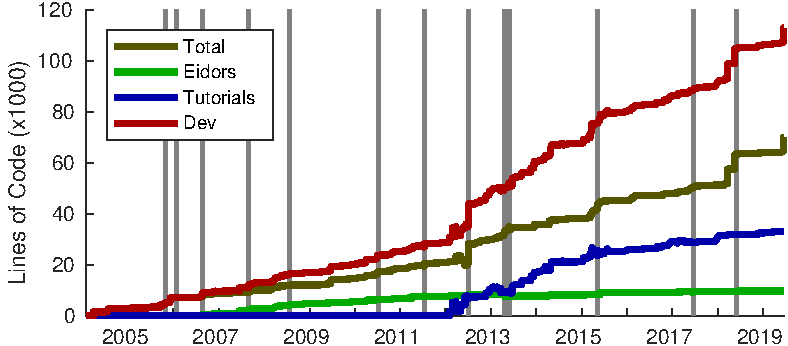
\includegraphics[width=.96\columnwidth]{fig_loc.pdf}
\caption{\label{fig:loc}%
%graph and table combo chart, including line for test code.
  Lines of Code (LoC) in Matlab files in the EIDORS code-base vs.\ time; Total
   (red), Eidors (i.e.\ release branch, brown), Tutorials (green), development code (blue).
   Releases are indicated by gray bars.
}
\end{figure}

\section{Discussion}
The structure of EIDORS has been relatively stable due, in part, to some early design choices:
a modular framework and data structure,
cross-platform support, integration of meshing,
tutorials, and the contributed data repository.
These aspects, along with an open source code-base, have enabled EIDORS to
maintain research relevance.
Presenting version 3.9!


\section*{Acknowledgements}
Recent funding for EIDORS development thanks to
NSERC Canada and EPSRC UK.

\footnotesize
\begin{thebibliography}{99}
\bibitem{eidors3p9}
   Adler A {\em et al}, ``EIDORS v3.9'',
   \href{http://dx.doi.org/10.5281/zenodo.583266}{DOI:10.5281/zenodo.583266},
    2017.
\bibitem{eidors3p8}
   Adler A {\em et al}, ``EIDORS v3.8'',
   \href{http://dx.doi.org/10.5281/zenodo.17559}{DOI:10.5281/zenodo.17559},
    2015.

\bibitem{grychtol2016}
   Grychtol B, Müller B, Adler A,
   {\em Physiol Meas}, 37:785--800, 2016.
\bibitem{braun2017}
   Braun F, Proença M, Solà J {\em et al}, \href{http://dx.doi.org/10.1109/TBME.2017.2659540}{IEEE T Biomed Eng}, 2017.
\bibitem{hansen2007}
   Hansen PC, {\em Numerical algorithms}, 46.2:189--194, 2007.

\bibitem{yerworth2016}
Yerworth R, Frerichs I, Bayford R, \href{http://dx.doi.org/10.1007/s10877-016-9920-y}{J Clin Monit Comput}, 2016.

\bibitem{boyle2016model2p5}
Boyle A, Adler A,
{\em Proc EIT2016}, p.100, Stockholm,  2016.

\bibitem{adler2016model}
Adler A, Lionheart WRB, 
%Model Reduction for FEM Forward Solutions
{\em Proc EIT2016}, p.116, Stockholm,  2016.

\bibitem{vauhkonen2001}
   Vauhkonen M, Lionheart WRB {\em  et al},
   {\em  Physiol Meas}, 22:107--111, 2001.
\bibitem{polydorides2002phd}
   Polydorides N,
%{\em Image Reconstruction Algorithms for Soft-Field Tomography},
 Ph.D. thesis, U Manchester, UK, 2002.
\bibitem{polydorides2002matlab}
   Polydorides N, Lionheart WRB,
   {\em Meas Sci Tech}, 13:1871--1883, 2002.
\bibitem{adler2005}
Adler A, Lionheart WRB,
%"EIDORS: Towards a community-based extensible software base for EIT." 6th Conference on Biomedical Applications of Electrical Impedance Tomography, London, UK. 2005.
{\em Proc EIT2015}, London, UK, 2015.
%
\bibitem{adler2006}
Adler A, Lionheart WRB,
{\em Physiol Meas} 27:S25--S42, 2006.

\bibitem{adler2008}
Adler A, Borsic A {\em et al},
%Simple FEMs aren't as good as we \ldots
{\em Proc EIT2008}, Hannover, NH, USA, 2008.
\bibitem{adler2015}
Adler A {\em et al}, %Alistair Boyle, Michael G Crabb, Hervé Gagnon, Bartłomiej Grychtol, Nolwenn Lesparre, William R.B. Lionheart,
\href{https://zenodo.org/record/17752}{\em Proc EIT2015}, p.19, 
 Neuchâtel, Switzerland, 2015.
\end{thebibliography}
\end{multicols}



\end{document}

